%%%%%%%%%%%%%%%%%%%%%%%%%%%%%%%%%%%%%%%%
%%% Compilation: PDFLaTeX BibTeX PDFLaTeX PDFLaTeX
%%% Dissertation: Master file                
%%% Style sheet: Antonio Machicao y Priemer   2025.04.13                                   
%%%%%%%%%%%%%%%%%%%%%%%%%%%%%%%%%%%%%%%%

\documentclass[
	a4paper,
	11pt,
	twoside,	% oneside, twoside
	%twoside=false, 	%No difference between left and right page
	openright,	% openleft, openright, openany
	BCOR=12mm,	% Correcting the bind margin
	%DIV=calc,	% Correcting Satzspiegel + DIV=last in localpackages
]{scrbook}

%% Cf. localpackages for further page settings


%% For a faster compilation use option: ``draft'' (e.g. graphics will not be displayed)
%\documentclass[draft,a4paper,11pt]{scrbook}

\setcounter{tocdepth}{4}
\setcounter{secnumdepth}{3}


%%%%%%%%%%%%%%%%%%%%%%%%%%%%%%%%%%
%%%  PACKAGES METADATA COMMANDS HYPHENATION            
%%%%%%%%%%%%%%%%%%%%%%%%%%%%%%%%%%

% put all additional packages, commands, etc. you need in the 
% following files. If you do not know what this might 
% mean, you can safely ignore this section

%%%%%%%%%%%%%%%%%%%%%%%%%%%%%%%%%%%%%%%%%%%%%%%%%%%%
%%%          MyP-Packages   2020.11.12   PhD thesis + PDFLaTeX
%%%%%%%%%%%%%%%%%%%%%%%%%%%%%%%%%%%%%%%%%%%%%%%%%%%%


\usepackage[utf8]{inputenc}

%%% Text in German:
%\usepackage[english,ngerman]{babel}

%% Text in English:
\usepackage[ngerman,english]{babel}

	%%% Change "Bibliography" into "References"
	\addto{\captionsenglish}{\renewcommand{\bibname}{References}}

	%\addto{\captionsenglish}{\renewcommand{\bibname}{Literatur}}
	
	%%% Change ''Abbildung'' into ''Abb.'' (for: babel)
	%\renewcommand{\thefigure}{\arabic{figure}}
	%\addto\captionsngerman{%
	%	\renewcommand{\figurename}{Abb.}%
	%}
	%\renewcommand{\figurename}{Abb.} 

	
%% TIPA encoding needs T3 & T1
\usepackage[T3,T1]{fontenc}

%% Fonts
%\usepackage{lmodern}

\usepackage{libertine}
	% change typewriter font to lmodern (smaller than tt in libertine)
	\renewcommand\ttdefault{lmtt}
	

%% For compatible mathematics (PDFLaTeX), it is recommended to use 
%\usepackage[libertine]{newtxmath}

%% Blind text: \blindtext \Blindtext \blindtext[5] \blindlist{itemize}[x] ...
\usepackage{blindtext}

%% ulem: Strike out
\usepackage[normalem]{ulem}  

%% graphicx: if gb4e is active PDFLaTeX does not accept files with underscore. PDFLaTeX only accepts files with .jpg, .png, .pdf endings
\usepackage{graphicx}


%%%%%%%%%%%%%%%%%%%%%%%%%%%%%%%%
%%%           Special Math-Symbols                   
%%%%%%%%%%%%%%%%%%%%%%%%%%%%%%%%

\usepackage{amsmath}
\usepackage{amsfonts}
\usepackage{amssymb}
\usepackage{MnSymbol}            %% Meaning brackets

\usepackage{pifont}                   %% checkmark

\usepackage{wasysym}              %% \Square \XBox \CheckedBox


%%%%%%%%%%%%%%%%%%%%%%%%%%%%%%%%
%%%         Tables & Lists & Columns            
%%%%%%%%%%%%%%%%%%%%%%%%%%%%%%%%

% Text in columns: \begin{multicols}{n} \columnbreak \end{multicols}
\usepackage{multicol}
%	\setlength{\columnsep}{.5cm}	

%% Tables with specified width
\usepackage{tabularx}

%% For complex tables
\usepackage{array}

%% For other tables
\usepackage{booktabs}

%% For more than one row in a table
\usepackage{multirow}

%% Special lists: itemize*
\usepackage{mdwlist}


%%%%%%%%%%%%%%%%%%%%%%%%%%%%%%%%
%%%          Coloured elements                  
%%%%%%%%%%%%%%%%%%%%%%%%%%%%%%%%
%Use xcolor before `gb4e'!
\usepackage{xcolor}


%%%%%%%%%%%%%%%%%%%%%%%%%%%%%%%%
%%%         TikZ                               
%%%%%%%%%%%%%%%%%%%%%%%%%%%%%%%%
% 
\usepackage{tikz}
\usetikzlibrary{patterns}


%%%%%%%%%%%%%%%%%%%%%%%%%%%%%%%%
%%%          Trees                               
%%%%%%%%%%%%%%%%%%%%%%%%%%%%%%%%
%% Forest must be loaded before `gb4e'
%% Package loaded with forest: tikz

\usepackage{forest}
	%% Needed for the "actual forest version"
	\useforestlibrary{linguistics}
	\forestapplylibrarydefaults{linguistics}



%%%%%%%%%%%%%%%%%%%%%%%%%%%%%%%%
%%%%       Attribute Value Matrices               
%%%%%%%%%%%%%%%%%%%%%%%%%%%%%%%%
\usepackage{langsci-avm}


%%%%%%%%%%%%%%%%%%%%%%%%%%%%%%%%
%%%          IPA                                 
%%%%%%%%%%%%%%%%%%%%%%%%%%%%%%%%
\usepackage[noenc,safe]{tipa}	


%%%%%%%%%%%%%%%%%%%%%%%%%%%%%%%%
%%%%          Verbatim                            
%%%%%%%%%%%%%%%%%%%%%%%%%%%%%%%%
%%`Listings' must be loaded before `gb4e', use `verbatim' otherwise
\usepackage{listings}

	\lstset{
		language=TeX,
		backgroundcolor=\color{lightgray},
		basicstyle={\footnotesize\ttfamily\color{blue}},
		showstringspaces=false,
		%	showspaces=false,
		breaklines=true,
		%	tabsize=2,
		columns=flexible
	}
	\lstset{literate=%
		{Ö}{{\"O}}1
		{Ä}{{\"A}}1
		{Ü}{{\"U}}1
		{ß}{{\ss}}2
		{ü}{{\"u}}1
		{ä}{{\"a}}1
		{ö}{{\"o}}1
	}
	

%%%%%%%%%%%%%%%%%%%%%%%%%%%%%%%%
%%%          Indices                            
%%%%%%%%%%%%%%%%%%%%%%%%%%%%%%%%

\usepackage{imakeidx}

\usepackage{acronym}


%%%%%%%%%%%%%%%%%%%%%%%%%%%%%%%%
%%%          Bibliography                        
%%%%%%%%%%%%%%%%%%%%%%%%%%%%%%%%

\usepackage[sectionbib]{natbib}
	\setlength{\bibsep}{0mm%pt plus 0.3ex
	}
	\setcitestyle{notesep={:~}}
	\setcitestyle{aysep={}} 


%%%%%%%%%%%%%%%%%%%%%%%%%%%%%%%%
%%%%          Settings of the page                
%%%%%%%%%%%%%%%%%%%%%%%%%%%%%%%%
%
%\KOMAoptions{
%DIV=last,	% Correcting Satzspiegel + DIV=calc in master (DIV=last after font)
%headsepline, 		%Line between heading and text (cf. Package scrpage2)
%}
%
%Headers & Footers
\usepackage[headsepline,
			%footsepline
			]{scrlayer-scrpage}
	\pagestyle{scrheadings}
	\clearscrheadfoot		%Clean all headers & footers
%	%%%%%%%%%%%%%%%%%%%%%%%%%	
%	%%One sided document:
%	%\ihead{Kopfzeile innen}
%	%\chead{Kopfzeile Mitte}
%	\ohead{\headmark}
%	\automark{section}
%	%\ifoot{Fußzeile innen}
%	%\cfoot{Fußzeile Mitte}
%	\ofoot{\pagemark} 
	%%%%%%%%%%%%%%%%%%%%%%%%%
	%%Two sided document:
	%\ihead{Kopfzeile innen}
	%\chead{Kopfzeile Mitte}
	\ohead{\headmark}
	\automark[chapter]{chapter}
	%\ifoot{Fußzeile innen}
	%\cfoot{Fußzeile Mitte}
	\ofoot{\pagemark} 
	%%%%%%%%%%%%%%%%%%%%%%%%%

%% (Vertical) Spacing
\usepackage{setspace}
	\onehalfspacing % to set the line spacing to 1.5. If you require single line spacing, comment this out.

%% Space for abbreviations 'i.d.R'
\usepackage{xspace}


%% Geometry: Setting up margins. This package must be loaded before `gb4e'
%\usepackage{geometry} 
%	\geometry{
%	left=3cm,
%	right=3cm,
%	%vmargin=3cm,
%	top=3cm,
%	bottom=3cm,
%	includeheadfoot
%	}


%% Footnote options: 
%% [bottom]: FN at the bottom, 
%% [hang] + 10pt: FN align
%% [splitrule]: If a FN is split across 2 pages, it adds a full-linelength line (http://tex.stackexchange.com/questions/32208/footnote-runs-onto-second-page)
\usepackage[bottom, hang, splitrule]{footmisc}
	\setlength\footnotemargin{0pt}
%	\setlength{\footnotesep}{.7\baselineskip}	%More spacing btw. FNs


%%%%%%%%%%%%%%%%%%%%%%%%%%%%%%%%%
%%%%%          Margin notes                        
%%%%%%%%%%%%%%%%%%%%%%%%%%%%%%%%%
\usepackage{todonotes}


%%%%%%%%%%%%%%%%%%%%%%%%%%%%%%%%
%%%           Examples                           
%%%%%%%%%%%%%%%%%%%%%%%%%%%%%%%%
\usepackage{langsci-gb4e}


%%%%%%%%%%%%%%%%%%%%%%%%%%%%%%%%
%%%          Hyperref & URL                      
%%%%%%%%%%%%%%%%%%%%%%%%%%%%%%%%
%\usepackage[hyphens]{url}
\usepackage[
bookmarksnumbered, %For numbered bookmarks in PDF
%	hidelinks %For links without colored borders
]{hyperref}

%%%%%%%%%%%%%%%%%%%%%%%%%%%%%%%%%%%%%%%%%%%%%%%%%%%%
%%%          MyP-Metadata   2020.11.12   PhD thesis + PDFLaTeX
%%%%%%%%%%%%%%%%%%%%%%%%%%%%%%%%%%%%%%%%%%%%%%%%%%%%


\title{\begin{Huge}NP-Arguments in NPs\end{Huge}}

\subtitle{An Analysis of German and Spanish Noun Phrases in Head-Driven Phrase Structure Grammar}


\dedication{For NN}

\author{Antonio Machicao y Priemer\\
	\url{http://www.linguistik.hu-berlin.de/staff/amyp}\\
	\href{mailto:mapriema@hu-berlin.de}{mapriema@hu-berlin.de}}


%\date{20/07/2019}


\publishers{Humboldt-Universität zu Berlin}


%% Properties of the PDF
\hypersetup{
	pdftitle={NP-Arguments in NPs},
	%	pdfsubject={Syntax},
	pdfauthor={Antonio Machicao y Priemer},
	pdfkeywords={syntax, semantics, quantifier, DP, NP, German, Spanish}
} %% needed if ``ch000-Frontpage'' is not used

%% hyphenation points for line breaks
%% Normally, automatic hyphenation in LaTeX is very good
%% If a word is mis-hyphenated, add it to this file
%%
%% add information to TeX file before \begin{document} with:
%% %% hyphenation points for line breaks
%% Normally, automatic hyphenation in LaTeX is very good
%% If a word is mis-hyphenated, add it to this file
%%
%% add information to TeX file before \begin{document} with:
%% %% hyphenation points for line breaks
%% Normally, automatic hyphenation in LaTeX is very good
%% If a word is mis-hyphenated, add it to this file
%%
%% add information to TeX file before \begin{document} with:
%% \include{localhyphenation}

\hyphenation{
%%English hyphenation	
	af-fri-cate
	af-fri-cates
	a-na-ly-sis
	a-na-ly-ses
	a-na-ly-se
	a-na-ly-sed
	com-ple-ment
	com-ple-ments
%% German hyphenation
	Ein-füh-rungs-ka-pi-tel
}

\hyphenation{
%%English hyphenation	
	af-fri-cate
	af-fri-cates
	a-na-ly-sis
	a-na-ly-ses
	a-na-ly-se
	a-na-ly-sed
	com-ple-ment
	com-ple-ments
%% German hyphenation
	Ein-füh-rungs-ka-pi-tel
}

\hyphenation{
%%English hyphenation	
	af-fri-cate
	af-fri-cates
	a-na-ly-sis
	a-na-ly-ses
	a-na-ly-se
	a-na-ly-sed
	com-ple-ment
	com-ple-ments
%% German hyphenation
	Ein-füh-rungs-ka-pi-tel
}

%%%%%%%%%%%%%%%%%%%%%%%%%%%%%%%%%%%%%%%%%%%%%%%%%%%%
%%%           MyP-Commands  2019.10.05    PhD thesis + PDF-LaTeX       
%%%%%%%%%%%%%%%%%%%%%%%%%%%%%%%%%%%%%%%%%%%%%%%%%%%%   

%%%%%%%%%%%%%%%%%%%%%%%%%%%%%%%%
%% Extra complex long definitions (e.g. X-bar) are in:
%% 
%%% localextracommands/lec-...

%%%%%%%%%%%%%%%%%%%%%%%%%%%%%%%%
%% ABBREVIATIONS
%%%%%%%%%%%%%%%%%%%%%%%%%%%%%%%%

%%%%%%%%%%%%%%%%%%%%%%%%%%%%%%%%
% Abbreviations in German
% package needed: xspace
% Short space in German abbreviations: \,	

\newcommand{\zB}{\mbox{z.\,B.}\xspace}



%%%%%%%%%%%%%%%%%%%%%%%%%%%%%%%%
%% TYPE SETTING
%%%%%%%%%%%%%%%%%%%%%%%%%%%%%%%%

%%%%%%%%%%%%%%%%%%%%%%%%%%%%%%%%
% German quotation marks:
\newcommand{\gqq}[1]{\glqq{}#1\grqq{}}		%double
\newcommand{\gq}[1]{\glq{}#1\grq{}}			%simple



%%%%%%%%%%%%%%%%%%%%%%%%%%%%%%%%
% Writing text with colour:
% package needed: xcolor
\newcommand{\blue}[1]{\textcolor{blue}{#1}}
\newcommand{\red}[1]{\textcolor{red}{#1}}

%%%%%%%%%%%%%%%%%%%%%%%%%%%%%%%%
%% Marking text with colour: 
%%% package needed: color
\newcommand{\clrr}[1]{\colorbox{red}{#1}}
\newcommand{\clry}[1]{\colorbox{yellow}{#1}}


%%%%%%%%%%%%%%%%%%%%%%%%%%%%%%%%
%% LINGUISTIC TYPOGRAPHY
%%%%%%%%%%%%%%%%%%%%%%%%%%%%%%%%



%%%%%%%%%%%%%%%%%%%%%%%%%%%%%%%%
%% Semantic types (<e,t>), features, variables and graphemes in angled brackets 

%%% types and variables, in math mode: angled brackets + italics + no space
%\newcommand{\type}[1]{$<#1>$}

%%% OR more correctly: 
%%% Types and Variables: chevrons! + text in math mode (italics + no space)
\newcommand{\type}[1]{$\langle #1 \rangle$} %% In Math Mode, only single types
\newcommand{\typem}[1]{\langle #1 \rangle } %% Mathmode extra, complex types

%%% Features and Graphemes: chevrons! + normal font
\newcommand{\ab}[1]{$\langle$#1$\rangle$} %% no italics
\newcommand{\abe}[1]{$\langle$\emph{#1}$\rangle$} %% italics

%%% Meaning brackets ([[xyz]]) + expression in italics
%% package needed: MnSymbol
\newcommand{\sem}[1]{$\lsem$\emph{#1}$\rsem$} %% italics
\newcommand{\semm}[1]{\lsem \textrm{\emph{#1}} \rsem} %% in math mode, italics

%% Denotational set
%% use in math mode: \ds{\typem{e,t}}
\newcommand{\ds}[1]{\textrm{D}_{#1}}

%% Predicates in formulae
%% use in math mode: \pred{Tisch} 
%\newcommand{\pred}[1]{\textrm{#1}'}  %% simple predicate with prime
\newcommand{\pred}[1]{\texttt{#1}}  %% simple predicate in type writer
\newcommand{\predO}[1]{\textrm{\textsc{#1}}} %% Operator in small caps

%% Presuppositions
\newcommand{\prspp}{$\gg$} 

%% Implicature
\newcommand{\implc}{$+ \mkern-5mu >$} 

%%%%%%%%%%%%%%%%%%%%%%%%%%%%%%%%
%% Function symbol in Beamer Class!
%% italics and serif
\newcommand{\func}{\emph{\textrm{f}}}
\newcommand{\gunc}{\emph{\textrm{g}}}
\newcommand{\chiF}[1]{\chi _{\textrm{#1}}} 

%%%%%%%%%%%%%%%%%%%%%%%%%%%%%%%%
%% HPSG: Features and Values!
\newcommand{\wert}[1]{\emph{#1}}        %Values & Types
\newcommand{\feat}[1]{\textsc{#1}}       %Features
\newcommand{\inx}[1]{\fbox{\footnotesize #1}}       %HPSG indices

%%%%%%%%%%%%%%%%%%%%%%%%%%%%%%%%
%% Subscript & Superscript: no italics inside math mode
\newcommand{\down}[1]{\textsubscript{#1}}
\newcommand{\downm}[1]{_{\textrm{#1}}}

\newcommand{\up}[1]{\textsuperscript{#1}}
\newcommand{\upm}[1]{^{\textrm{#1}}}

%%%%%%%%%%%%%%%%%%%%%%%%%%%%%%%%%
%% Shorter Underline
\DeclareTextCommand{\_}{T1}{\leavevmode \kern.06em\vbox{\hrule width.4em}}

%%%%%%%%%%%%%%%%%%%%%%%%%%%%%%%%
%% (Syntactic) Trees
% package needed: forest
% with option: linguistics

%%% Setting for complex trees
%% "bottom word" is the old "sn edges", but the later is used as default (idk y)
\forestset{
	bottom word/.style={for tree={parent anchor=south, child anchor=north,align=center,base=bottom,where n children=0{tier=word,inner xsep=0pt,outer sep=0pt}{}}}, 
	%
	background tree/.style={for tree={text opacity=0.2,draw opacity=0.2,edge={draw opacity=0.2}}}
}

%% Use HideWd for translations when using roof and the translations are longer than the original text
%% https://tex.stackexchange.com/questions/167978/smaller-roofs-for-forest
\newcommand\HideWd[1]{%
	\makebox[0pt]{#1}%
}



%%%%%%%%%%%%%%%%%%%%%%%%%%%%%%%%
%% NOTES & BOX
%%%%%%%%%%%%%%%%%%%%%%%%%%%%%%%%

%%%%%%%%%%%%%%%%%%%%%%%%%%%%%%%%
%% Outputbox
\newcommand{\outputbox}[1]{\noindent\fbox{\parbox[t][][t]{0.98\linewidth}{#1}}\vspace{0.5em}}

%%%%%%%%%%%%%%%%%%%%%%%%%%%%%%%%
%% TO DO NOTES
% package needed: todonote
\newcommand{\todolit}[1]{\todo[color=green!40]{LIT: #1}}
\newcommand{\todored}[1]{\todo[color=red!60]{#1}}


%%%%%%%%%%%%%%%%%%%%%%%%%%%%%%%%
%% Chapter Notes: \begin{chnote}\end{chnote}
%%% package needed: 
%
\newenvironment{chnote}{
	\color{blue}
	%	\noindent \paragraph*{CHAPTER NOTES} 
	\begin{itemize*}
	}
	%	
	{
	\end{itemize*} 
}


%%%%%%%%%%%%%%%%%%%%%%%%%%%%%%%%
%% Index newcommand:
%%% package needed: imakeidx package
\newcommand{\is}[1]{\index{#1}{#1}}

%for terms of implementations (files, code, etc.)
\newcommand{\ist}[1]{\index{#1}{\texttt{#1}}}

%for terms in math mode
\newcommand{\ism}[1]{\index{$#1$}{$#1$}}   


%%%%%%%%%%%%%%%%%%%%%%%%%%%%%%%%
%% Theoretical Abbreviations & Commands
%% in English: 

%%%% Theories
\newcommand{\GB}{\index{Government \& Binding Theory (GB)}{GB}}	

\newcommand{\GPSG}{\index{Generalized Phrase Structure Grammar (GPSG)}{\ac{GPSG}}}	

%%%% HPSG Terminology & Commands
\newcommand{\attr}[1]{\index{attribute!\textsc{#1}}{\textsc{#1}}}
	

%%%% HPSG Principles:
\newcommand{\CaseP}{\index{principle!Case Principle (CaseP)}{CaseP}}


%%%% Further Terminology & Commands
\newcommand{\throle}{\index{theta role}{theta role}}
\newcommand{\throles}{\index{theta role}{theta roles}}


%%%%%%%%%%%%%%%%%%%%%%%%%%%%%%%%
%% Corpora
% 
\newcommand{\ESCOW}{\citetext{ESCOW \citeyear{SchaeferR&Co12a}}}

\makeindex %% if you don't use an index comment this out


%%%%%%%%%%%%%%%%%%%%%%%%%%%%%%%%%%
%%%             PREAMBLE'S END                  
%%%%%%%%%%%%%%%%%%%%%%%%%%%%%%%%%%

\begin{document}       


%%%%%%%%%%%%%%%%%%%%%%%%%%%%%%%%%%
%%%     FRONTMATTER
%%%%%%%%%%%%%%%%%%%%%%%%%%%%%%%%%%


%%% FRONTPAGE: Use ch000-Frontpage OR use maketitle 
%%%%%%%%%%%%%%%%%%%%%%%%%%%%%%%%%%%%%%%%%%%%%%%%%
%% Compile the master file
%% this file contains the frontpage only
%% Template for theis (Antonio Machicao y Priemer)
%%%%%%%%%%%%%%%%%%%%%%%%%%%%%%%%%%%%%%%%%%%%%%%%%


\thispagestyle{empty}


\vspace{5.6cm}

%% complete page centered
\begin{center}

%% Title
\begin{minipage}{.99\textwidth}
	\begin{center}

	\begin{huge}
	\textbf{NP-Arguments in NPs}
	\end{huge}

	\end{center}
\end{minipage}


\vspace{.5cm}

%% Subtitle
\begin{minipage}{.99\textwidth}
	\begin{center}
	\doublespacing

	\begin{Large}
	An Analysis of German and Spanish Noun Phrases\\
	in Head-Driven Phrase Structure Grammar
	\end{Large}

	\end{center}
\end{minipage}


\vspace{1.4cm}


\begin{minipage}{.99\textwidth}
	\begin{center}

	
\includegraphics[scale=1]{graphics/husiegelswgross}

	\end{center}
\end{minipage}


\vspace{1.4cm}


\begin{minipage}{.99\textwidth}
\centering
	Dissertation\\
	zur Erlangung des akademischen Grades 


\vspace{.3cm}


	\textbf{Doktor der Philosophie (Dr.\ phil.)}


\vspace{.3cm}


	eingereicht an der Sprach- und literaturwissenschaftlichen Fakultät\\
	der Humboldt-Universität zu Berlin


\vspace{.5cm}


	von\\
	M.\,A. Maria-Luise Mustermann\\
	geboren am 20.07.1999 in Berlin.
\end{minipage}


\vspace{.9cm}


\begin{minipage}[][][t]{.99\textwidth}
\centering	
	\begin{minipage}[][][t]{.48\textwidth}
	Prof.\ Dr.\ Dr.\ Helene Musterfrau
	
	Präsidentin
	
	der Humboldt-Universität zu Berlin
	\end{minipage} 
	%
	\begin{minipage}[][][t]{.03\textwidth}
	~
	\end{minipage}	
	%
	\begin{minipage}[][][t]{.46\textwidth}
		Prof.\ Dr.\ Ulrike Pérez-Schmidt
		
		Dekanin
		der Sprach- und 
		
		literaturwissenschaftlichen Fakultät
	\end{minipage}
\end{minipage}


\vspace{.85cm}


\begin{minipage}{.99\textwidth}

	~Gutachter:innen:

	\begin{enumerate*}
		\item Prof.\ Dr.\ Anita Musterfrau
		\item Prof.\ Dr.\ Jonas Mustermann
	\end{enumerate*}

\end{minipage}


\end{center}

%\maketitle                
%%\thispagestyle{empty}


\frontmatter


\tableofcontents      


\listoffigures
	\addcontentsline{toc}{chapter}{List of Figures}


\listoftables
	\addcontentsline{toc}{chapter}{List of Tables}


%%% (un)comment if you have (not) preface, acknowledgements or abbreviations

%	%%%%%%%%%%%%%%%%%%%%%%%%%%%%
%%%%%%%%%%%%%%%%%%%%%%%%%%%%
\chapter{Preface}
%%%%%%%%%%%%%%%%%%%%%%%%%%%%


\blindtext[5] 

	%%%%%%%%%%%%%%%%%%%%%%%%%%%%
%%%%%%%%%%%%%%%%%%%%%%%%%%%%
\chapter{Acknowledgements}
\label{sec:thanks}
%%%%%%%%%%%%%%%%%%%%%%%%%%%%



Thank you! 

\Blindtext %% adds `blind' text useful in testing new classes and packages

 	%%%%%%%%%%%%%%%%%%%%%%%%%%%%
%%%%%%%%%%%%%%%%%%%%%%%%%%%%
\chapter{Abbreviations}

%% Check the documentation of the package acronym
%% https://www.ctan.org/pkg/acronym
%%%%%%%%%%%%%%%%%%%%%%%%%%%%


All abbreviations used in this work -- except the ones for glosses in examples -- are listed below. For glossed examples, the norms and abbreviations supplied by the  \emph{Leipzig Glossing Rules} \citep[cf.][]{LeipzigGloss15a} were used.



%\begin{multicols}{2}
%\setlength{\columnseprule}{.5pt}
\begin{acronym}[n--sg--strong]
%
%A
	\acro{acc}[\textit{acc}]{accusative}
%
%B
%
%C
	\acro{CP}{complementiser phrase}
%
%D
	\acro{dat}[\textit{dat}]{dative}
%
%E
%
%F
%
%G
%
%H
%
%I
	\acro{IPA}{International Phonetic Alphabet}	
%
%L
%
%M	
%
%N
%
%O
%
%P
%
%Q
%
%R
%
%S
%
%T
%
%U
%
%V
%
%W	
%
%X
%
%Y
%
%Z	
\end{acronym}
%\end{multicols}



\mainmatter         


%%%%%%%%%%%%%%%%%%%%%%%%%%%%%%%%%%
%%%       CHAPTERS
%%%%%%%%%%%%%%%%%%%%%%%%%%%%%%%%%%

%%%%%%%%%%%%%%%%%%%%%%%%%%%%
%%%%%%%%%%%%%%%%%%%%%%%%%%%%
\chapter{Introduction}
\label{ch:Introduction}
%%%%%%%%%%%%%%%%%%%%%%%%%%%%


\Blindtext
 

%%%%%%%%%%%%%%%%%%%%%%%%%%%%
%%%%%%%%%%%%%%%%%%%%%%%%%%%%
\chapter{Theory}
\label{ch:Theory}
%%%%%%%%%%%%%%%%%%%%%%%%%%%%


\Blindtext

%%%%%%%%%%%%%%%%%%%%%%%%%%%%
%%%%%%%%%%%%%%%%%%%%%%%%%%%%
\chapter{Analysis}
\label{ch:Analysis}
%%%%%%%%%%%%%%%%%%%%%%%%%%%%


\Blindtext %% adds `blind' text useful in testing new classes and packages


%%%%%%%%%%%%%%%%%%%%%%%%%%%%
\chapter{Conclusions}
\label{ch:Conclusions}
%%%%%%%%%%%%%%%%%%%%%%%%%%%%


\Blindtext

%%%%%%%%%%%%%%%%%%%%%%%%%%%%
%%%%%%%%%%%%%%%%%%%%%%%%%%%%
\chapter{\LaTeX\ Help}
\label{ch:Help}
%%%%%%%%%%%%%%%%%%%%%%%%%%%%


In this chapter, I will show you how to use some of the commands and packages in the template for PhD theses. The following topics will be explained:

\begin{itemize}
	\item What is in the file \texttt{localcommands} and how can I use the commands? (Sec.~\ref{ch:Commands})
	
	\item How can I work with the package \texttt{langsci-gb4e} for examples? (Sec.~\ref{ch:Examples})
		
	\item How can I insert figures and tables with floating environments? (Sec.~\ref{ch:FigTab})
	
	\item Which entry types can I use for bibliographic information? (Sec.~\ref{ch:BibEntries} \& \ref{ch:CitationCommands})
		
	\item Abbreviations and indices (Sec.~\ref{ch:Indices})

	\item How can I add personal to-do notes to my text? (Sec.~\ref{ch:Notes})
\end{itemize}

All packages mentioned here are loaded in \texttt{texfiles/localpackages}.
Take into account that this is not an introduction into \LaTeX . For a short \LaTeX\  introduction (in German), see \citet{Freitag&MyP15a}.


%%%%%%%%%%%%%%%%%%%%%%%%%%%%
%%%%%%%%%%%%%%%%%%%%%%%%%%%%
\section{Own commands}
\label{ch:Commands}
%%%%%%%%%%%%%%%%%%%%%%%%%%%%

In the file \texttt{texfiles/localcommands} you can define your own commands. I have pre-defined some commands such that you can see how that works.

\begin{itemize}
	\item \verb|\zB| renders the German abbreviation \zB (for `for example'), with a protected blank between ``z.'' and ``B.''.
	
	\item \verb|\gqq{argument}|  renders the German double quotation marks, as in \gqq{argument}.
	
	\item \verb|\gq{argument}|  renders the German single quotation marks, as in \gq{argument}.
	
	\item The commands \verb|\red{argument}| and \verb|\blue{argument}| render text in blue or red, e.g.\ \red{argument}, \blue{argument}.
	
	\item The commands \verb|\clrr{argument}| and \verb|\clry{argument}| render text marked with red  or yellow, e.g.\ \clrr{argument}, \clry{argument}.
\end{itemize}


%%%%%%%%%%%%%%%%%%%%%%%%%%%%
%%%%%%%%%%%%%%%%%%%%%%%%%%%%
\section{Examples}
\label{ch:Examples}
%%%%%%%%%%%%%%%%%%%%%%%%%%%%


In this document, the package \texttt{langsci-gb4e} is loaded%
	%
	\footnote{All packages are loaded in the file \texttt{texfiles/localpackages}.} %
	%
for creating example environments.
It is a slightly modified version of \texttt{gb4e}, see the \texttt{gb4e} manual \citep{Kolb&Co10a} or \citet{Freitag&MyP15a}) for further explanations.
\texttt{langsci-gb4e} can be used with the same \LaTeX \ syntax as \texttt{gb4e}:


\begin{lstlisting}
\begin{exe}
\ex This is an example.
\ex This is the second example.
  \begin{xlist}
    \ex embedded examples with different numbering
    \ex These examples are numbered with letters.
    \ex another example numbered with letters
  \end{xlist}
\end{exe}
\end{lstlisting}


\noindent \texttt{langsci-gb4e} also provides a somewhat simpler syntax:

\begin{lstlisting}
\ea This is an example.
\ex This is the second example.
  \ea embedded examples with different numbering
  \ex These examples are numbered with letters.
  \ex another example numbered with letters
  \z   
\z
\end{lstlisting}


The result in both cases is the same:

\ea This is an example.

\ex This is the second example.

	\ea embedded examples with different numbering
	
	\ex These examples are numbered with letters.
	
	\ex another example numbered with letters
	\z   
\z


%%%%%%%%%%%%%%%%%%%%%%%%%%%%
%%%%%%%%%%%%%%%%%%%%%%%%%%%%
\section{Figures and Tables}
\label{ch:FigTab}
%%%%%%%%%%%%%%%%%%%%%%%%%%%%


There is a floating environment for figures. It is floating but you can (try to) fix%
	%
	\footnote{If there is not enough place where you want to position the graphic, \LaTeX\ will choose a different place, e.g.\ at the top of the next page.} %
	%
the figure on a position with the option \texttt{[h]}. The environment is helpful to center figures using the command \verb|\centering| and to add captions that are listed in the List of Figures.%
	%
	\footnote{For more on figures, tables, and captions, see \citet{Freitag&MyP15a}.} %
	%

By using the command \verb|\includegraphics| from the package \texttt{graphicx} you can include graphics. All you have to do is indicate the graphic's file path (see the Figure~\ref{fig:Frege}).


\begin{lstlisting}
\begin{figure}[h]
  \centering
  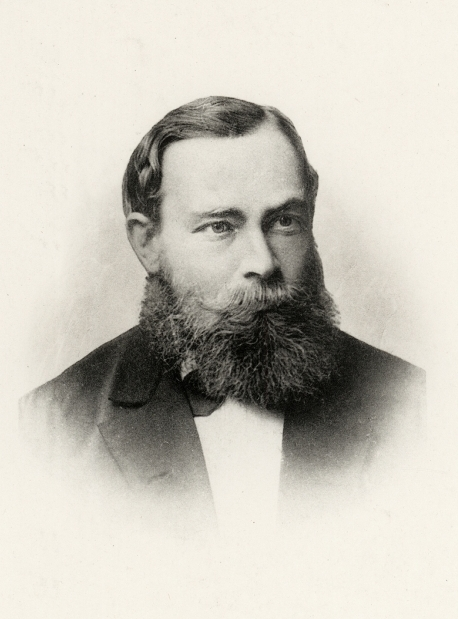
\includegraphics[scale=.45]{graphics/Young-Frege}
  \caption{Young Frege}
  \label{fig:Frege}
\end{figure}
\end{lstlisting}


\begin{figure}[h]
	\centering
	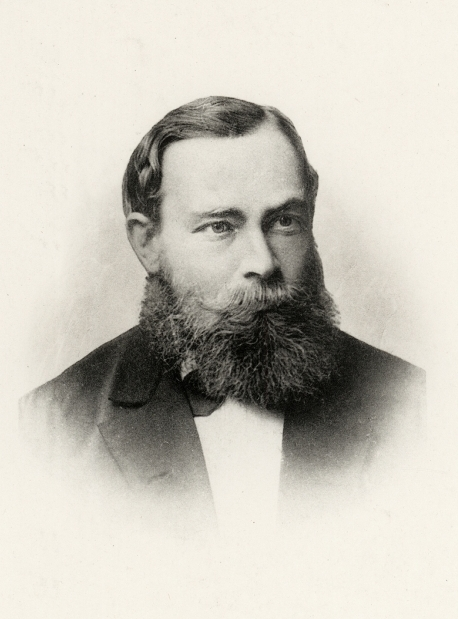
\includegraphics[scale=.45]{graphics/Young-Frege}
	\caption{Young Frege}
	\label{fig:Frege}
\end{figure}


\noindent It works in the same way for tables.


\begin{lstlisting}
\begin{table}[h]
  \centering
  \begin{tabular}{l|l}
    Figure & Table \\
    \hline
    test & test \\
  \end{tabular}
  \caption{Test table}
\end{table}
\end{lstlisting}


\begin{table}[h]
	\centering
	\begin{tabular}{l|l}
		Figure & Table \\
		\hline
		test & test \\
	\end{tabular}
	\caption{Test table}
\end{table}


%%%%%%%%%%%%%%%%%%%%%%%%%%%%
%%%%%%%%%%%%%%%%%%%%%%%%%%%%
\section{Examples for different bibliographical entries}
\label{ch:BibEntries}
%%%%%%%%%%%%%%%%%%%%%%%%%%%%


In order to see which information you need in your Bib\TeX\ file for different entry types%
	%
	\footnote{See also \url{https://en.wikipedia.org/wiki/BibTeX} or \citet{Freitag&MyP15a}.} %
	%
(e.g.\ article, book, manuscript, etc.), check the file \texttt{texfiles/literature}.%
	%
	\footnote{The file \texttt{texfiles/literature} is the Bib\TeX\ file for this document. You can introduce your entries there.} %
	%
If you want to see the output for every specific entry type (e.g.\ \texttt{phdthesis} vs.\ \texttt{book}), take a look at the bibliography of this PDF.


\begin{itemize}
	\item PhD Thesis: \citet{Abney87a}
	
	\item Article in an edited book: \citet{Ackema15a}
	
	\item Book: \citet{Adger04a}
	
	\item Edited book: \citet{MyP&Co14b}
	
	\item Article in a journal: \citet{Barwise&Co81a}
	
	\item Article in an online journal or database:
	\citet{Kolb&Co10a}
	
	\item Unpublished work / manuscript: \citet{LeipzigGloss15a}
	
	\item Published work without author, using a key, i.e.\ an abbreviation for the citation (this can be used e.g.\ for corpora or dictionaries): \citep{DR17a}
	
	\item Published entry in an encyclopedia (online): \citet{MyP18b}
\end{itemize}


%%%%%%%%%%%%%%%%%%%%%%%%%%%%
%%%%%%%%%%%%%%%%%%%%%%%%%%%%
\section{Examples for different citation commands with \texttt{natbib}}
\label{ch:CitationCommands}
%%%%%%%%%%%%%%%%%%%%%%%%%%%%

The package \texttt{natbib} (loaded in \texttt{texfiles/localpackages}) provides different commands for citations. You can find the IDs for every bibliography entry in the file \texttt{texfiles/literature}, but they are also being suggested as soon as you type in one of the \verb|\cite| commands.


\vspace{.5cm}


\begin{footnotesize}

\begin{tabular}{p{7cm}|p{5.6cm}}
	\textbf{input} & \textbf{output} \\
	\midrule
	\verb|\citep{Heim&Kratzer00a}| & {\citep{Heim&Kratzer00a}} \\
	
	\verb|\citep[cf.][4--5]{Heim&Kratzer00a}| & {\citep[cf.][4--5]{Heim&Kratzer00a}} \\
	
	 \verb|\citet{Heim&Kratzer00a}| & {\citet{Heim&Kratzer00a}} \\

	\verb|\citep[cf.][]{Heim&Kratzer00a}| & {\citep[cf.][]{Heim&Kratzer00a}} \\

	\verb|\citep[56--76]{Heim&Kratzer00a}| & {\citep[56--76]{Heim&Kratzer00a}} \\

	\verb|\citealp[56]{Heim&Kratzer00a}| & {\citealp[56]{Heim&Kratzer00a} }\\

	\verb|\citealt[43ff]{Heim&Kratzer00a}| &{\citealt[43--45]{Heim&Kratzer00a}} \\

	\verb|\citep{Heim&Kratzer00a,Abney87a}|  & {\citep{Heim&Kratzer00a,Abney87a}} \\
\end{tabular}

\end{footnotesize}


%%%%%%%%%%%%%%%%%%%%%%%%%%%%
%%%%%%%%%%%%%%%%%%%%%%%%%%%%
\section{Abbreviations and indices}
\label{ch:Indices}
%%%%%%%%%%%%%%%%%%%%%%%%%%%%


For further information about \index{index}indices, take a look at the documentation of the package \texttt{imakeidx}%
	%
	\footnote{\url{https://ctan.org/pkg/imakeidx}.} %
	%
and the Wikipedia page for indices.%
%
\footnote{\url{https://en.wikibooks.org/wiki/LaTeX/Indexing}} %
%

For abbreviations, the package \texttt{acronym}%
%
\footnote{\url{https://ctan.org/pkg/acronym}.} %
%
is very useful and easy to implement. First the abbreviations are defined (see Section Abbreviations) and then used with the command \verb|\ac{acronym}|.  The pre-defined acronyms in the Section Abbreviations are: 

\begin{itemize}
\item \ac{acc}, 
\item \ac{CP}, 
\item \ac{dat},  
\item \ac{IPA} 
\end{itemize}


%%%%%%%%%%%%%%%%%%%%%%%%%%%%
%%%%%%%%%%%%%%%%%%%%%%%%%%%%
\section{Notes}
\label{ch:Notes}
%%%%%%%%%%%%%%%%%%%%%%%%%%%%


If you want to write preliminary margin notes, \todo{This note is orange.} you can use the command \verb|\todo|.%
	%
	\footnote{Take a look at the documentation of the package \url{https://ctan.org/pkg/todonotes}. You can customise your own to-do notes.} %
	%

%%%%%%%%%%%%%%%%%%%%%%%%%%%%
%%%%%%%%%%%%%%%%%%%%%%%%%%%%
\section{Links in the PDF}
%%%%%%%%%%%%%%%%%%%%%%%%%%%%

In the PDF file several elements are framed in red or green. These elements are links, the coloured frames will not appear in the print version of your document. In case you do not want to see the frames, just comment in the option \texttt{hidelinks} for the package \texttt{hyperref} in the file \texttt{texfiles/localpackages}.



%%%%%%%%%%%%%%%%%%%%%%%%%%%%%%%%%%
%%%             References                      
%%%%%%%%%%%%%%%%%%%%%%%%%%%%%%%%%%

\begin{singlespace}

%% For two sided documents
\cleardoublepage 

%%% For one sided documents
%\clearpage

\phantomsection %this allows hyperlink in ToC to work
\addcontentsline{toc}{chapter}{References}


%%%% Bibliography style in German
%\bibliographystyle{texfiles/deChicagoMyP}

%%% Bibliography style in English
%\bibliographystyle{texfiles/enChicagoMyP}
%% OR
\bibliographystyle{texfiles/unified}

\bibliography{texfiles/literature}


%%%%%%%%%%%%%%%%%%%%%%%%%%%%%%%%%%
%%%                INDICES
%%%%%%%%%%%%%%%%%%%%%%%%%%%%%%%%%%

%% if you don't use an index comment the following commands UNTIL \printindex out 

%% For two sided documents
\cleardoublepage 

%%% For one-sided documents
%\clearpage

\phantomsection %this allows hyperlink in ToC to work
\addcontentsline{toc}{chapter}{Index} 


\printindex 


\end{singlespace}


\end{document}